\subsection{Smart Owl}
    \subsubsection{Definición}
      \paragraph{La función principal del Smart Owl es la obtención de la información de diversas fuentes, tanto estáticas y dinámicas.}
      \paragraph{Todas la información que se encontrará en las bases de datos de tipo MX será obtenida a través de Smart Owl, muchas de las fuentes no cuentan con los datos climatológicos completos, principalmente las gubernamentales como: CONAGUA, INEGI o SMN, por citar algunas.}
      \paragraph{Considerando esa problematica, Smart Owl buscará y tratará de resolver la información de los campos faltantes tomando como base distintas fuentes de datos, algunas establecidas y otras de tipo gubernamental.}
      \paragraph{También se tomará información de fuentes que tipo dinámica,es decir, cuya información suele ser actualizada en entre periodos de una o dos horas. Estas fuentes suelen contar con RESTFul API's para consumo de forma programática.}
      \paragraph{El modelo de datos final podrá ser entonces persistido después de que haya sido resuelto completa o parcialmente. Se llevará el control de los metadatos considerando su origen, su fecha y algunos tags relacionados los que proveen la información.}
    \newpage
     \subsection{Dificultades}
      \paragraph{El desarrollo del módulo tiene su complejidad en las fuentes de datos que tienen estructuras muy variadas, por lo que para tener un primer avance se han programado las pruebas unitarias y la funcionalidad para la extracción y estandarización de la información de cada fuente.}
      \paragraph{Hasta ahora se cuenta con 3 recursos: los archivos que provee la CONAGUA (Comisión Nacional del Agua), la información de Weather Underground y la API de Forecast.io.}
      \subsection{Tecnologías de desarrollo}
      \paragraph{Para la construcción de todos los módulos se está haciendo uso del lenguaje de programación Groovy. Las pruebas unitarias se definieron con la ayuda de Spock Framework y la construcción del proyecto se está ejecutando de manera automática con Gradle.}
    \newpage
      \begin{landscape}
      \subsubsection{Diagrama por bloques.}
        \paragraph{A continuación se mostrará el diagrama por bloques que define la estructura de Smart Owl.}
        \begin{figure}[b!]
        \centering
        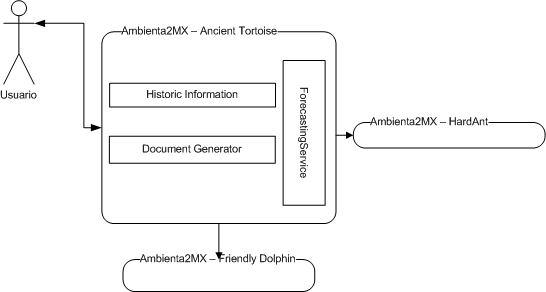
\includegraphics[width=22.5cm,height=12cm]{./images/DiagramaAncientTortoise.png}
        \caption{Diagrama General de Smart Owl}
      \end{figure}
      \end{landscape}
      \newpage
    \paragraph{A continuación se muestran los diagramas de secuencia planteados para el funcionamiento del módulo mencionado.}
    \begin{center}
      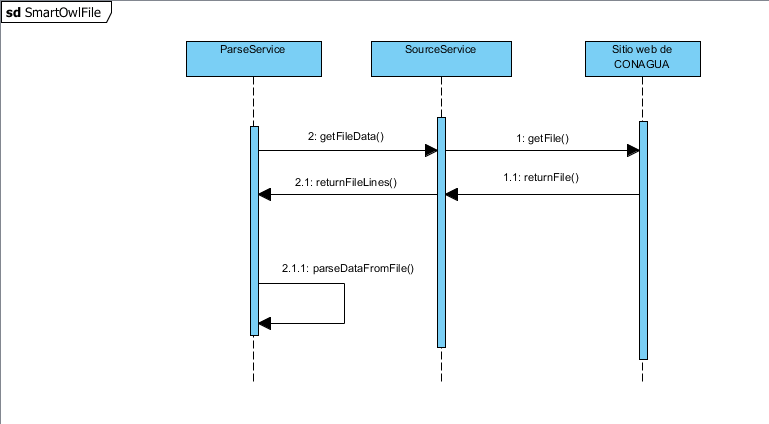
\includegraphics[width=14cm,height=9cm]{./images/SmartOwlSequenceDiagram}
    \end{center}
    \begin{center}
      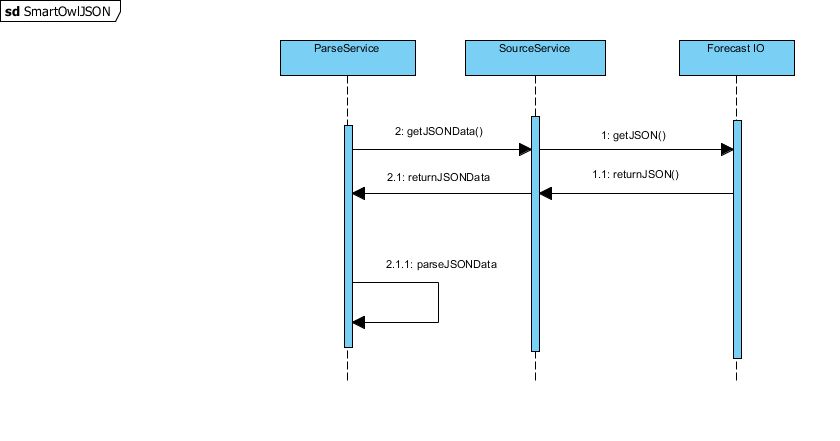
\includegraphics[width=14cm,height=9cm]{./images/SmartOwlSequenceDiagram2}
    \end{center}
    \subsubsection{Diagrama por bloques}